\chapter{Grupos}

\section{Operaciones binarias}

\begin{definition}{Operación binaria}{op-bin}
    Sea \(X\) un conjunto. Una operación binaria en \(X\) es una aplicación \(*:X\times X\to X\). Por lo general escribimos \( * (a,b) = a * b\).
\end{definition}

\begin{remark}
    En general, si por el contexto se sobreentiende que una operación es binaria, se simplifica el lenguaje hablando simplemente de operaciones. De igual manera, normalmente se omite el conjunto sobre el que está definida la operación.
\end{remark}

\begin{definition}{Tipos de operaciones}{tipos-op}
    Una operación $*$ se dice
    \begin{itemize}
        \item \textbf{Conmutativa} si $x * y = y * x$ para todo $x,y\in X$.
        \item \textbf{Asociativa} si $x * (y * z) = (x * y) * z$ para todo $x,y,z \in X$.
    \end{itemize}
\end{definition}

\begin{definition}{Terminología sobre elementos}{term-elem}
    Un elemento \(x\in X\) se dice que es:
    \begin{itemize}
        \item \textbf{Neutro por la izquierda (neutro por la derecha)} si \(x*y=y\) para todo \(y\in X\) (\(y*x=y\) para todo \(y\in X\)).
        
        \item \textbf{Cancelable por la izquierda (cancelable por la derecha)} si para cada dos elementos distintos \(a \neq b\) de \(X\) se verifica \(x*a\neq x*b\) (\(a*x\neq b*x\)).
        
        \item \textbf{Neutro} si es neutro por la derecha y por la izquierda.

        \item \textbf{Cancelable} si es cancelable por la izquierda y por la derecha.
    \end{itemize}

    Supongamos que \(e\) es un elemento neutro de \(X\) con respecto a \(*\). Sean \(x\) e \(y\) elementos de \(X\). Decimos que \(x\) es simétrico de \(y\) por la izquierda y que \(y\) es simétrico de \(x\) por la derecha con respecto a \(*\) si se verifica \(x*y=e\). En este contexto decimos que $x$ es:
    \begin{itemize}
        \item \textbf{Simétrico} de $y$ si lo es por ambos lados. En tal caso decimos que $x$ es invertible, siendo $y$ su inverso ($y = x^{-1}$ si el inverso es único).
    \end{itemize}
\end{definition}

\begin{example}{}{}
    Si $x$ es cancelable por la izquierda, entonces para cualesquiera $a,b \in X$ se tiene
    \[
    x * a = x * b \implies a = b
    \]
\end{example}

\begin{proofbox}
    Supongamos que $x * a = x * b$, si $a = b$ ya hemos terminado. En caso contrario, $a$ y $b$ son elementos distintos, y, como $x$ es cancelable por la izquierda, entonces debe ser $x * a \neq x * b$, pero eso contradice la suposición inicial, luego ha de ser $a = b$.
\end{proofbox}

\begin{example}{}{}
Si $x$ es cancelable por la derecha entonces, para cualesquiera $a,b \in X$ se tiene
    \[
    a * x = b * x \implies a = b
    \]
\end{example}

\begin{remark}
    Notemos que esta caracterización no es más que el contrarrecíproco de la primera definición que hemos dado de elemento cancelable. 
\end{remark}

\begin{definition}{Tipos de conjuntos con operaciones}{tipos-conj-op}
    Un par \((X,*)\) formado por un conjunto y una operación \(*\) decimos que es un:
    \begin{itemize}
        \item \textbf{Semigrupo} si \(*\) es asociativa.
        
        \item \textbf{Monoide} si es un semigrupo que tiene un elemento neutro con respecto a \(*\).
        
        \item \textbf{Grupo} si es un monoide y todo elemento de \(X\) es invertible con respecto a \(*\).
        
        \item \textbf{Grupo abeliano} si es un grupo y \(*\) es conmutativa.
    \end{itemize}
\end{definition}

\begin{example}{}{conjuntos-op-binarias}
    Si tomamos la suma de elementos sobre distintos conjuntos de números obtenemos un ejemplo de cada uno de los tipos de conjuntos con operaciones:
    \begin{enumerate}
        \item $(\N \setminus \{ 0 \},+)$ es un semigrupo, ya que la suma es asociativa, pero no tiene neutro.
        \item $(\N,+)$ es un monoide, ya que la suma es asociativa y tiene el 0 como neutro.
        \item $(\Z,+)$ es un grupo, ya que la suma es asociativa, tiene neutro y todos los elementos tienen inverso. De hecho, como la suma es conmutativa es un grupo abeliano.
    \end{enumerate}
\end{example}

\begin{example}{Grupo no abeliano}{grupo-no-abeliano}
    Un ejemplo de grupo no abeliano es $GL_n(\R)$ si $n \geq 2$. $GL_n(\R)$ es el grupo de las matrices invertibles $n\times n$ con entradas reales, donde la operación es la multiplicación de matrices.
\end{example}

\begin{proofbox}
    En primer lugar, es inmediato que la operación es asociativa. También es fácil ver que tiene elemento neutro, la matriz identidad $I_n$. Si tomamos una matriz cualquiera $A\in GL_n(\R)$ esta ha de tener inversa, por lo que su elemento inverso es $A^{-1}$ que claramente pertenece a $GL_n(\R)$.

    Finalmente, para ver que el grupo no es conmutativo notemos que para $n=2$ podemos tomar las matrices
    \[
    A = \begin{pmatrix} 1 & 1 \\ 0 & 1 \end{pmatrix}, B = \begin{pmatrix} 1 & 1 \\ 1 & 0 \end{pmatrix}
    \]
    ambas invertibles por tener determinante no nulo, que verifican
    \[
    AB = \begin{pmatrix} 2 & 1 \\ 1 & 0 \end{pmatrix} \neq BA = \begin{pmatrix} 1 & 2 \\ 1 & 1 \end{pmatrix}.
    \]
    En el caso de que sea $n > 2$ podemos tomar matrices de la forma
    \[
    A' = \begin{pmatrix} A & 0 \\ 0 & I_{n-2} \end{pmatrix}, B' = \begin{pmatrix} B & 0 \\ 0 & I_{n-2} \end{pmatrix}
    \]
    cuyo producto no conmuta por las propiedades de la multiplicación de matrices por bloques.
\end{proofbox}

\begin{example}{}{}
    Sean $A$ un conjunto y sea $X=A^{A}$ el conjunto de las aplicaciones de $A$ en $A$. Probar que la composición de aplicaciones define una operación asociativa en $X$ para la que la identidad $1_{X}$ es neutro. Esto prueba que $(A^{A},\circ)$ es un monoide.
\end{example}

\begin{proposition}{}{prop-operaciones}
    Sea $*$ una operación en un conjunto $X$.

    \begin{enumerate}
    
    \item Si $e$ es un neutro por la izquierda y $f$ es un neutro por la derecha de $X$ con respecto a $*$, entonces $e = f$. En particular, $X$ tiene a lo sumo un neutro.
    
    \item Supongamos que $(X, *)$ es un monoide y sea $a \in X$.
    \begin{enumerate}
        \item Si $x$ es un simétrico por la izquierda de $a$ e $y$ es un simétrico por la derecha de $a$, entonces $x = y$. Por tanto, en tal caso $a$ es invertible y tiene a lo sumo un simétrico.
        
        \item Si $a$ tiene un simétrico por un lado entonces es cancelable por ese mismo lado. En particular, todo elemento invertible es cancelable.
    \end{enumerate}
    \end{enumerate}
\end{proposition}

\begin{proofbox}
    (1) Como $e$ es neutro por la izquierda y $f$ es neutro por la derecha tenemos
    \[
    f = e * f = e.
    \]
    (2a) Ahora suponemos que $(X, *)$ es un monoide. Por (1), $(X, *)$ tiene un único neutro que vamos a denotar por $e$. Como $x$ es inverso por la izquierda de $a$ e $y$ es inverso por la derecha de $a$, usando la propiedad asociativa, tenemos que
    \[
    y = e * y = (x * a) * y = x * (a * y) = x * e = x.
    \]
    (2b) Supongamos que $a$ es un elemento de $X$ que tiene un inverso por la izquierda $b$ y que $a * x = a * y$ para $x, y \in X$. Usando la asociatividad una vez más concluimos que
    \[
    x = e * x = (b * a) * x = b * (a * x) = b * (a * y) = (b * a) * y = e * y = y.
    \]
\end{proofbox}

\begin{remark}
    Por la proposición anterior si $X$ es un monoide cada elemento invertible $a$ tiene un único inverso que denotaremos $a^{-1}$. 
\end{remark}

\subsection{Subconjuntos y operaciones}

Sea $*$ una operación en un conjunto $A$ y sea $B$ un subconjunto de $A$. Decimos que $B$ es cerrado con respecto a $*$ si para todo $a, b \in B$ se verifica que $a * b \in B$. En tal caso podemos
considerar $*$ como una operación en $B$ que se dice inducida por la operación en $A$.

\begin{itemize}
\item Un subsemigrupo de un semigrupo es un subconjunto suyo que con la misma operación es un semigrupo.

\item Un submonoide de un monoide es un subconjunto suyo que con la misma operación es un monoide con el mismo neutro.

\item Un subgrupo de un grupo es un subconjunto suyo que con la misma operación es un grupo.
\end{itemize}

\clearpage
\section{Definiciones y ejemplos}

\begin{definition}{Grupo}{grupo}
    Un grupo es una pareja \((G,\cdot)\), formada por un conjunto no vacío \(G\) junto con una operación binaria, que denotaremos por \(\cdot\), que satisface los siguientes axiomas:
    \begin{enumerate}
    \item {(Asociativa)} \((a\cdot b)\cdot c = a\cdot(b\cdot c)\), para todo \(a,b,c\in G\).
    \item {(Neutro)} Existe un elemento \(e\in G\), llamado {elemento neutro del grupo}, tal que \(e\cdot a = a = a\cdot e\), para todo \(a\in G\).
    \item {(Inverso)} Para todo \(a\in G\) existe otro elemento \(a^{-1}\in G\), llamado {elemento inverso} de \(a\), tal que \(a\cdot a^{-1} = e = a^{-1}\cdot a\).
    \end{enumerate}

    Si además se verifica el siguiente axioma se dice que el grupo es {abeliano} o {conmutativo}:

    \begin{enumerate}
    \setcounter{enumi}{3}
    \item {(Conmutativa)} \(a\cdot b = b\cdot a\), para todo \(a,b\in G\).
    \end{enumerate}
\end{definition}

Demostraremos ahora algunas propiedades de los grupos.

\begin{lemma}{Propiedades básicas de grupos}{prop-grupos}
    Sea \((G,\cdot)\) un grupo.
    \begin{enumerate}
    \item {(Unicidad del neutro)} El neutro de \(G\) es único y lo denotaremos \(e\). De hecho, si \(a,b\in G\) satisfacen que \(a\cdot b = a\) ó \(b\cdot a = a\) entonces \(b = e\).
    \item {(Unicidad del inverso)} El inverso de un elemento \(a\) de \(G\) es único y lo denotaremos \(a^{-1}\). De hecho, si \(e\) es el neutro de \(G\) y \(a,b\in G\) satisfacen \(a\cdot b = e\) ó \(b\cdot a = e\) entonces \(b = a^{-1}\).
    \item {(Propiedad Cancelativa)} Todo elemento de \(G\) es cancelativo.
    \item Para todo \(a,b\in G\), las ecuaciones \(a\cdot X = b\) y \(X\cdot a = b\) tienen una única solución en \(G\).
    \item \((a\cdot b)^{-1} = b^{-1}\cdot a^{-1}\).
    \end{enumerate}
\end{lemma}

\begin{proofbox}
    \begin{enumerate}
    \item
        Haremos solo el caso por la derecha, en efecto, si $a \cdot b = a$ entonces
        \[
        b = e \cdot b = a^{-1} \cdot a \cdot b = a^{-1} \cdot a = e.
        \]

    \item
        De nuevo hacemos solo el caso \(a\cdot b = e\)
        \[
        a^{-1} = a^{-1} \cdot e = a^{-1} \cdot a \cdot b = e \cdot b = b.
        \]

    \item
        Sea $x \in G$, entonces $x$ debe ser cancelable puesto que en caso contrario existirían $a,b \in G$ con $a \neq b$ tales que $x \cdot a = x \cdot b$, pero entonces
        \[
        a = e \cdot a = x^{-1} \cdot x \cdot a = x^{-1} \cdot x \cdot b = e \cdot b = b
        \]
        una contradicción.

    \item
        Sean $a,b \in G$ arbitrarios y $x,y$ dos soluciones cualesquiera, entonces
        \[
        x = e \cdot x = a^{-1} \cdot a \cdot x = a^{-1} \cdot b
        \]
        y de igual manera
        \[
        y = e \cdot y = a^{-1} \cdot a \cdot y = a^{-1} \cdot b
        \]
        luego $x=y$. Para la otra ecuación se razona igual. Notemos que también hemos demostrado la existencia de una solución ($x = a^{-1} \cdot b$).

    \item
        Basta realizar un sencillo cálculo y aplicar el apartado 2
        \[
        (a \cdot b) \cdot (b^{-1} \cdot a^{-1}) = a \cdot b \cdot b^{-1} \cdot a^{-1} = a \cdot e \cdot a^{-1} = a \cdot a^{-1} = e.
        \]

    \end{enumerate}
\end{proofbox}

\subsection{Ejemplos}

\begin{example}{Grupo trivial}{grupo-trivial}
    Sea \(X\) un conjunto y consideremos la aplicación identidad $1_X: X \to X$ tal que $1_X(x) = x$ para todo $x \in X$. Entonces el conjunto $T = \{1_X\}$ con la operación de composición es un grupo $(T, \circ)$ que llamaremos el grupo trivial (lo denotaremos $1$).
    
    En general, podríamos haber definido este grupo como un único elemento $\{x\}$ con la operación descrita por $x \cdot x = x$.
\end{example}

En términos de grupos de transformaciones, el grupo trivial de $X$ es el grupo de transformaciones más pequeño que podemos construir. Que en efecto se trata de un grupo es inmediato.

\begin{example}{Grupo simétrico}{grupo-simetrico}
    Sean \(X\) un conjunto y \(S_X\) el conjunto de todas las biyecciones de \(X\) en sí mismo. Entonces \((S_X, \circ)\) es un grupo, llamado {grupo simétrico} o {grupo de las permutaciones} de \(X\).
\end{example}

En términos de grupos de transformaciones, el grupo de permutaciones de $X$ es el grupo de transformaciones más grande que podemos construir. Probemos ahora que en efecto es un grupo.

\begin{proofbox}
    Prescindiremos del uso de $\circ$ para simplificar la notación.
    \begin{enumerate}
        \item Asociativa: sean $f,g,h$ biyecciones, dado $x \in X$ cualquiera
        \[
            ((fg)h) x = (fg)(h(x)) = f(g(h(x))) = f(gh(x)) = (f(gh))x \implies (fg)h = f(gh)
        \]
        \item Neutro: basta considerar la aplicación identidad $id(x) = x$.
        \item Inverso: claramente el inverso de una biyección cualquiera $f$ es su inversa $f^{-1}$, que verifica
        \[
        (f f^{-1})(x) = f(f^{-1}(x)) = x
        \]
        luego $ff^{-1} = id$.
    \end{enumerate}
\end{proofbox}

\begin{remark}
    En general $S_X$ no es un grupo abeliano.
\end{remark}

\begin{example}{Producto de grupos}{prod-grupos}
    Si \((G, *)\) y \((H, *)\) son dos grupos, entonces el {producto directo} \(G \times H\) es un grupo en el que la operación viene dada componente a componente:
    \[
    (g_1, h_1) \cdot (g_2, h_2) = (g_1 * g_2, h_1 * h_2).
    \]
    Más generalmente, si \((G_i)_{i\in I}\) es una familia arbitraria de grupos, entonces el producto directo \(\prod_{i\in I} G_i\) tiene una estructura de grupo en el que el producto se realiza componente a componente. Para más información ver la Definición \ref{defn:producto-cartesiano}.
\end{example}

Probemos que el producto directo de dos grupos es un grupo:

\begin{proofbox}
    \begin{enumerate}
        \item Asociativa:
        \begin{align*}
            ((g_1, h_1) \cdot (g_2, h_2)) \cdot (g_3, h_3) &= (g_1 * g_2, h_1 * h_2) \cdot (g_3, h_3) = (g_1 * g_2 * g_3, h_1 * h_2 * h_3) = \\
            &= (g_1, h_1) \cdot (g_2 * g_3, h_2 * h_3) = (g_1, h_1) \cdot ((g_2, h_2) \cdot (g_3, h_3))
        \end{align*}
        donde hemos usado la asociatividad de los grupos $G, H$.
        \item Neutro: basta considerar el elemento $(e_G, e_H)$ donde $e_G$ es el neutro de $G$ y $e_H$ el de $H$.
        \item Inverso: claramente el inverso de un elemento cualquiera $(g_1, h_1)$ es $(g_1^{-1}, h_1^{-1})$, que verifica
        \[
        (g_1, h_1) \cdot (g_1^{-1}, h_1^{-1}) = (g_1 * g_1^{-1}, h_1 * h_1^{-1}) = (e_G, e_H).
        \]
    \end{enumerate}
\end{proofbox}

\begin{example}{Tabla de Cayley}{tabla-cayley}
    Dado un grupo finito podemos construir lo que llamaremos su tabla de Cayley (también llamada tabla de multiplicación o de suma, dependiendo del nombre que le demos a la operación del grupo). Esta tabla se obtiene disponiendo cada uno de los elementos del grupo tanto por columnas como por filas y calculando sus productos. Si el grupo tiene 2 elementos $a,b$ la tabla será de la forma:
    \begin{center}
        \begin{tabular}{c | c | c}
            $\cdot$ & $a$ & $b$ \\
            \hline
            $a$ & $a \cdot a$ & $a \cdot b$  \\ 
            \hline
            $b$ & $b \cdot a$ & $b \cdot b$ \\
            \hline
        \end{tabular}
    \end{center}

    Como ejemplo concreto, la tabla del grupo $\Z_3$ (enteros módulo 3) es la siguiente:
    \vspace{10pt}
    \begin{center}
        \begin{tabular}{c | c | c | c}
            $+$ & $0$ & $1$ & $2$ \\
            \hline
            $0$ & $0$ & $1$ & $2$ \\ 
            \hline
            $1$ & $1$ & $2$ & $0$ \\ 
            \hline
            $2$ & $2$ & $0$ & $1$ \\ 
            \hline
        \end{tabular}
    \end{center}
\end{example}

\subsection{El grupo diédrico}

Veamos ahora un grupo con especial significado geométrico. Consideremos un polígono regular de \(n\) lados y las transformaciones que lo dejan invariantes (rotaciones y reflexiones), a las que llamaremos simetrías. La composición de dos simetrías de un polígono regular es nuevamente una simetría de este objeto. Considerando la composición de simetrías como operación binaria, esto le da a las simetrías la estructura algebraica de un grupo finito.

La siguiente tabla de Cayley muestra el efecto de la composición en el grupo diédrico de orden 6, \(D_3\) -- las simetrías de un triángulo equilátero. Aquí, \(r_0\) denota la identidad, \(r_1\) y \(r_2\) denotan rotaciones en sentido antihorario de \(120^\circ\) y \(240^\circ\) respectivamente, mientras que \(s_0\), \(s_1\) y \(s_2\) denotan reflexiones a través de las tres líneas mostradas en la imagen adyacente.

\begin{figure}[h]
    \centering
    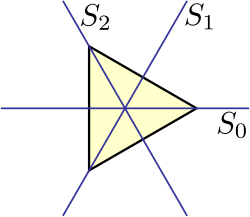
\includegraphics[width=5cm]{img/diedrico.png}
\end{figure}

\[
\begin{array}{c|cccccc}
\circ & r_0 & r_1 & r_2 & s_0 & s_1 & s_2 \\
\hline
r_0 & r_0 & r_1 & r_2 & s_0 & s_1 & s_2 \\
r_1 & r_1 & r_2 & r_0 & s_1 & s_2 & s_0 \\
r_2 & r_2 & r_0 & r_1 & s_2 & s_0 & s_1 \\
s_0 & s_0 & s_2 & s_1 & r_0 & r_2 & r_1 \\
s_1 & s_1 & s_0 & s_2 & r_1 & r_0 & r_2 \\
s_2 & s_2 & s_1 & s_0 & r_2 & r_1 & r_0 \\
\end{array}
\]

Por ejemplo, \(s_2 s_1 = r_1\), porque la reflexión \(s_1\) seguida de la reflexión \(s_2\) resulta en una rotación de \(120^\circ\). El orden de los elementos que denotan la composición es de derecha a izquierda, reflejando la convención de que el elemento actúa sobre la expresión a su derecha. La operación de composición no es conmutativa.

El siguiente ejemplo abstrae y generaliza el concepto de grupo diédrico prescindiendo de la interpretación geométrica.

\begin{example}{Grupo diédrico}{diedrico}
    Para cada número natural positivo \(n\) definimos un grupo formado por \(2n\) elementos
    \[
    D_n = \{1, a, a^2, \ldots, a^{n-1}, b, ab, a^2b, \ldots, a^{n-1}b\}
    \]
    en el que la multiplicación viene dada por la siguiente regla:
    \[
    (a^{i_1} b^{j_1})(a^{i_2} b^{j_2}) = a^{[i_1 + (-1)^{j_1} i_2]_n} b^{[j_1 + j_2]_2}
    \]
    con notación como en el ejemplo anterior. Este grupo se llama {grupo diédrico de orden \(2n\)}.

    El grupo diédrico infinito \(D_\infty\) está formado por elementos de la forma \(a^n b^m\), con \(n \in \mathbb{Z}\) y \(m = 0, 1\) con el producto \((a^{i_1} b^{j_1})(a^{i_2} b^{j_2}) = a^{i_1 + (-1)^{j_1} i_2} b^{[j_1 + j_2]_2}\).
\end{example}

Si ahora consideramos únicamente las rotaciones que dejan invariante un polígono de \(n\) lados obtenemos otro grupo, en este caso con \(n\) elementos, cada uno de ellos correspondiente a rotar por un múltiplo de $\frac{360^\circ}{n}$. El siguiente ejemplo abstrae este grupo de rotaciones.

\begin{example}{Grupo cíclico}{ciclico}
    Para cada número natural positivo \(n\) definimos un grupo \(C_n\) formado por \(n\) elementos
    \[
    C_n = \{1, a, a^2, \ldots, a^{n-1}\},
    \]
    donde \(a\) es un símbolo, y en el que la multiplicación viene dada por la siguiente regla:
    \[
    a^i a^j = a^{[i+j]_n}
    \]
    donde \([x]_n\) denota el resto de dividir \(x\) entre \(n\). Este grupo se llama {cíclico de orden \(n\)}.

    También definimos el {grupo cíclico infinito} como el conjunto \(C_\infty = \{a^n : n \in \mathbb{Z}\}\), donde \(a\) es un símbolo y consideramos \(a^n = a^m\) si y solo si \(n = m\), y en el que el producto viene dado por \(a^n \cdot a^m = a^{n+m}\).
\end{example}

\begin{remark}
    Es fácil notar la similitud entre $C_n$ y $\Z_n$, así como entre $C_\infty$ y $\Z$. Más tarde formalizaremos esta intuición probando que estos grupos son equivalentes (isomorfos).
\end{remark}